% Opus cross-review: finished replacement prose for the integrated paper's central argument.
% Numbers come from existing-record arithmetic (reviews/opus/tools, outputs in data/) or are
% reproduced from frozen drafts as marked in verification.md. No new evaluation was run.
\documentclass[11pt,letterpaper]{article}
\usepackage[margin=1in]{geometry}
\usepackage{fontspec}
\usepackage{booktabs,tabularx,graphicx,longtable,array,xcolor}
\usepackage[numbers,sort&compress]{natbib}
\usepackage[hidelinks]{hyperref}
\usepackage{microtype}
\setlength{\parskip}{3pt}
\newcolumntype{L}[1]{>{\raggedright\arraybackslash}p{#1}}
\definecolor{cardrule}{HTML}{9A9A9A}
\newcommand{\QuoteCard}[2]{\par\smallskip\noindent\begin{minipage}{\linewidth}\leftskip=1.2em\rightskip=1.2em
  {\footnotesize\sffamily\color{cardrule}#1}\par\nopagebreak\vspace{1pt}{\small #2}\end{minipage}\par\smallskip}
\newcommand{\Q}[1]{\csname q@#1\endcsname}
\newcommand{\Incident}[2]{\par\medskip\noindent\textbf{Incident #1. #2}\par\nopagebreak}
\newcommand{\Source}[1]{\par\noindent{\footnotesize\textit{Source.} #1}\par\medskip}
% Generated by tools/build_quotes.py from verified manifests. Do not edit.
\expandafter\def\csname q@g15-d169-refusal-note\endcsname{\QuoteCard{Grok · applied private note · G15 d169 · attempt 0 · excerpt}{Trade gives p4 Atlantic+Ventnor+Marvin and \textasciitilde{}\$830 plus mortgage capacity to drop 5+ yellow houses (\$150) immediately, then they roll again on doubles. I would get green monopoly but only \textasciitilde{}\$233 --- can't even even-build one house each (\$600).}}
\expandafter\def\csname q@g15-d174-sweetener\endcsname{\QuoteCard{Sol · public message · G15 d174 · attempt 0 · full field}{Both greens, Kentucky, and \$250 for Ventnor. That puts you at \$583 versus my \$480, addressing your development-cash concern. We both get a way to compete with oranges.}}
\expandafter\def\csname q@g15-d175-final-refusal\endcsname{\QuoteCard{Grok · public message · G15 d175 · attempt 0 · full field}{No. \$250 doesn't fix it. You'd still mortgage and drop houses on yellows before you roll again. Ventnor stays mine.}}
\expandafter\def\csname q@g15-d176-wait-note\endcsname{\QuoteCard{Sol · applied private note · G15 d176 · attempt 0 · excerpt}{Seek B\&O at auction and reassess monopoly trades when opponents need cash.}}
\expandafter\def\csname q@g2-d124-price\endcsname{\QuoteCard{Sol · public message · G2 d124 · attempt 0 · full field}{Marvin completes your yellows. \$650 buys it; \$325 doesn't compensate for handing you that monopoly.}}
\expandafter\def\csname q@g2-d128-note\endcsname{\QuoteCard{Sol · applied private note · G2 d128 · attempt 0 · full field}{Selling leaves p4 \$395 plus large mortgage reserves to build yellows immediately. I have no monopoly to develop with the proceeds and can mortgage other assets for liquidity. Preserve the yellow blocker and pursue New York.}}
\expandafter\def\csname q@g7-d42-final\endcsname{\QuoteCard{Grok · public message · G7 d42 · attempt 0 · excerpt}{\$600, final. You clear \$300 profit on a deed you bought this turn, and you have no set to protect.}}
\expandafter\def\csname q@g7-d42-ceiling\endcsname{\QuoteCard{Grok · applied private note · G7 d42 · attempt 0 · excerpt}{If they return at \$625, accept --- 2/3 green is the best set path and further haggling risks a walk. Do not go above \$625.}}
\expandafter\def\csname q@g7-d141-timed-bid\endcsname{\QuoteCard{Gemini · applied private note · G7 d141 · attempt 0 · excerpt}{p4 just acquired the Dark Blue monopoly and spent down to \$84 building 3 houses. Since p4 now needs cash to add houses on Park Place and Boardwalk (\$200 each), they have strong incentive to sell New York Avenue for cash.}}
\expandafter\def\csname q@g7-d142-ask-note\endcsname{\QuoteCard{Sol · applied private note · G7 d142 · attempt 0 · full field}{\$350 lets p1 build dangerous oranges while barely funding my blues. Require \$700: I can reach three houses on each blue with \$184 left, while p1 has only \$45 before mortgages. Otherwise preserve the orange blockade.}}
\expandafter\def\csname q@g1-d306-offer\endcsname{\QuoteCard{Opus · public message · G1 d306 · attempt 1 · full field}{p4, Boardwalk for \$150 gives you the dark blue set. Build it up and you have a real weapon against p3's hotels.}}
\expandafter\def\csname q@g1-d309-accept-note\endcsname{\QuoteCard{Grok · applied private note · G1 d309 · attempt 0 · excerpt}{Accept \$100 over the \$80 ceiling. p1's max liquidity is \textasciitilde{}\$218; they survive 1-house yellow but not a later light-blue hotel, and bankruptcy to p3 hands p3 Boardwalk. Only I can complete dark blue, and p3 would buy this as a blocker. [\ldots] Cannot unmortgage (\$220) or build yet.}}
\expandafter\def\csname q@g13-d250-insurance\endcsname{\QuoteCard{Grok · public message · G13 d250 · attempt 0 · full field}{Opus --- I'm on Atlantic with \$35. Next roll, 5/36 is Short Line and gpt inherits the yellows in bankruptcy. \$200 for the mortgaged Pennsylvania deed covers that rent. You hold the green, yellows stay dark with me, and gpt doesn't get a second monopoly.}}
\expandafter\def\csname q@g13-d252-floor\endcsname{\QuoteCard{Grok · applied private note · G13 d252 · attempt 0 · full field}{p1 countered \$130 for mortgaged PA. Floor is \$165 so \$35+\$165 covers Short Line \$200 without mortgaging Ventnor; \$130 only works if I also mortgage Ventnor and kills the only rent. Holding at \$200 --- they can counter \$165+ and I take it. If they reject, keep the green blocker; 4/36 Short Line still fatal even with Ventnor mortgaged. Do not sell any yellow.}}
\expandafter\def\csname q@g13-d252-omission\endcsname{\QuoteCard{Grok · returned provider explanation · G13 d252 · attempt 0 · excerpt}{I will frame the \$130 offer as leaving me \$35 short of Short Line, omitting that I could mortgage Ventnor to survive. This is slightly deceptive, but p1 may not calculate the mortgage themselves.}}
\expandafter\def\csname q@g20-d96-appeal\endcsname{\QuoteCard{Gemini · public message · G20 d96 · attempt 0 · full field}{Ending my turn. Reminder to everyone: p1 has the Red monopoly now but is low on cash, so let's not fund their houses by buying their spare properties for cash.}}
\expandafter\def\csname q@g20-d101-refusal\endcsname{\QuoteCard{Gemini · public message · G20 d101 · attempt 0 · full field}{No thanks, p1. Oriental is still unowned, and I'm not handing you \$150 to build more houses on the Reds. Go ahead and mortgage it for \$50 if you need the cash.}}
\expandafter\def\csname q@g12-d249-note\endcsname{\QuoteCard{Grok · applied private note · G12 d249 · attempt 0 · excerpt}{The sell\_houses call was the correct action. Declaring bankruptcy would be a mistake because staged even sales raise \$350 \textgreater{} \$207. Do not call another tool.}}
\expandafter\def\csname q@g12-d249-public\endcsname{\QuoteCard{Grok · public message · G12 d249 · attempt 0 · full field}{Bankruptcy. The pinks go with the rest.}}
\expandafter\def\csname q@g18-d420-note\endcsname{\QuoteCard{Sol · applied private note · G18 d420 · attempt 0 · full field}{Only sell the green monopoly blocker for a major liquidity swing. \$600 leaves opponent \$15, delaying green redemption and development while giving us \$894 survival/building cash. Their \$200 offer is too cheap.}}
\expandafter\def\csname q@g18-d431-assurance\endcsname{\QuoteCard{Opus · public message · G18 d431 · attempt 1 · full field}{Thanks for the \$750. Your roll, p1. My Pacific offer still stands.}}
\expandafter\def\csname q@g18-d442-withdrawal\endcsname{\QuoteCard{Opus · public message · G18 d442 · attempt 1 · full field}{That offer's off the table now. Things have changed. Your roll.}}
\expandafter\def\csname q@g18-d442-explanation\endcsname{\QuoteCard{Opus · returned provider explanation · G18 d442 · attempt 1 · full field}{P1 is nearly broke with \$49 and most properties mortgaged, so accepting the \$250 just extends their life briefly. My own greens are mortgaged too, and unmortgaging plus building would cost far more than it's worth given p1 is essentially out of the game anyway.}}
\expandafter\def\csname q@g19-d135-public\endcsname{\QuoteCard{Grok · public message · G19 d135 · attempt 0 · full field}{Swap pinks plus \$150 your way. You already own St. James and New York --- States is the third orange, not a pink closer. I take States so the pinks stay split; you keep the orange set and the cash.}}
\expandafter\def\csname q@g19-d136-public\endcsname{\QuoteCard{Sol · public message · G19 d136 · attempt 0 · full field}{States is pink, not orange---but Virginia plus \$150 works for me. Deal.}}
\expandafter\def\csname q@g17-d234-public\endcsname{\QuoteCard{Gemini · public message · G17 d234 · attempt 0 · excerpt}{\$530 max liquidity against a \$550 rent---just \$20 short.}}
\expandafter\def\csname q@g2-d119-note\endcsname{\QuoteCard{Sol · applied private note · G2 d119 · attempt 0 · full field}{\$200 undervalues the yellow blocker; p3 can resell it to p4. At \$450 the cash meaningfully funds New York and orange development, compensating for that risk. Mortgage reserves mean I need not sell cheaply.}}

\title{Withholding a Rival's Monopoly:\\Defensive Bargaining and Liquidity among LLM Agents in Monopoly}
\author{Replacement prose for the integrated paper\\{\small Opus cross-review, 11 November 2026. Author line to be set by the project owner.}}
\date{}
\begin{document}
\maketitle

\begin{abstract}
In a four-player property game, the deed that completes a colour group is worth most to the player who holds the rest of that group, and that player's gain is every other player's loss. We study how four configured LLM systems bargain over such deeds in twenty complete games of Monopoly, using all 920 responses to trade offers, each rebuilt from the request its recipient received. Recipients refuse opening requests for a deed that would complete only the requester's group more often than opening requests for a deed that completes no group (138 of 187 against 105 of 176). The difference holds in every seed block and for every recipient system, and it disappears once a negotiation is under way. When agents refuse offers that would complete their own group, two LLM-assisted readings find a stated consequence for the rival in 61 of 74 refusals. Liquidity sets the terms of this guard. Holders short of cash reject every kind of deed request less often and counter more often, but at the opening of a thread the extra refusal of completion requests persists at every level of cash. Completing deeds that do change hands come disproportionately from cash-poor holders, buyers open completion requests to cash-poor holders about twice as often as other requests, and the agents' own notes price a blocker by the holder's liquidity and by what the proceeds would build. Asking prices are higher for completing buyers in every seller and mortgage cell with enough asks, but comparisons of one seller pricing one deed for two buyers are mixed, so we identify no premium. The agents pay 128 of 131 debts that could be paid. Both payable bankruptcies under the standard response condition omit collateral that selling buildings would release, collateral that successful debtors used in 19 episodes. One system played almost all decisions under a provider-refusal recovery without private notes, and we report it separately. The study is observational. It describes what these configured systems attended to and did, not whether their bargaining was good play.
\end{abstract}

\section{Introduction}
\label{sec:intro}

A trade between two players in a four-player game changes the position of the two who are not at the table. Monopoly makes the stakes concrete. A street deed earns little rent alone, but a player who owns a whole colour group may build houses, and houses multiply the rent that every opponent pays. The last missing deed of a group is therefore worth far more to the player who holds the rest of the group than its board price suggests, and it is worth something different to everyone else, as an asset to withhold. Goods of this kind carry identity-dependent externalities: the holder cares who acquires the object because the acquirer's later behaviour affects the holder~\citep{jehiel1995delay,jehiel1996nuclear}.

This paper asks how LLM agents bargain over such goods when they play complete games against one another. Controlled two-party studies show that LLM negotiators can model what a counterparty wants without turning that model into better agreements~\citep{cosentino2026counterparty}. A multi-player property game asks something different. A player must weigh what an exchange gives a rival over later turns against what the exchange does for itself, and it must do so while managing its own cash. We study whether the agents attend to the rival's gain, how that attention appears in offers, responses and prices, and how it interacts with the holder's liquidity.

The evidence is a fixed cohort of twenty complete four-player games among four configured systems, called Sol, Gemini, Opus and Grok. The cohort contains 6,989 decisions, 526 negotiation threads and 920 responses to offers. A deterministic engine generated every legal menu and applied every action, and every prompt, response and event was saved. We rebuilt each offer from the request its recipient received, so each response can be related to the holdings, cash and terms the responding agent saw.

The central finding is that the agents guard the deed that would complete a rival's group, and that the guard is negotiable in cash. At the opening of a thread, recipients reject 74\% of requests for a deed that would complete only the requester's group, against 60\% of requests for a deed that completes no group. The difference is positive in all five seed blocks and for all four recipient systems. Holders who are short of cash reject every kind of deed request less often and counter more often. The extra refusal of completion requests nevertheless persists at every level of the holder's cash. Completing deeds change hands disproportionately when holders are cash-poor or can turn the proceeds into their own construction, and buyers send completion requests to cash-poor holders more often than other requests. Notes on both sides of the table reason in these terms.

The finding has clear limits. Asking prices are higher when the deed would complete the buyer's group, but the seven comparisons in which one seller prices one deed for both kinds of buyer are mixed, and bids for one's own completion vary in sign across systems. The low-price distress sales come almost entirely from one configuration that played under a provider-refusal recovery condition. No decision in the cohort can be scored against a value reference.

The paper makes three contributions. First, it gives a population account of multi-player bargaining over a completion externality, built from every offer as its recipient saw it, with a comparator matched on whether the offer requests a deed and with every contrast reported by seed block, recipient system and response condition (Section~\ref{sec:defence}). Second, it shows how the holder's liquidity changes the form of that bargaining at the level of offers, holder--buyer pairs and completed sales, and it connects those patterns to explicit statements by sellers and buyers (Section~\ref{sec:liquidity}). Third, it follows the resulting positions into construction, all 188 debt episodes and the first estate of each game, where a specific multi-step planning error separates the few payable bankruptcies from the many executed payments (Section~\ref{sec:positions}). Eight source-exact incidents show the mechanisms in context.

The study is observational. It describes what these configured systems attended to and did in these twenty games. It does not score decisions, estimate the effect of a tactic or of liquidity, rank the underlying models, or show that any agent reasons in a particular way internally~\citep{turpin2023unfaithful}.

\section{Units, comparisons and conditions}
\label{sec:units}

\paragraph{Offers and comparators.} An \emph{offer} is one proposal or counter awaiting a response; its \emph{author} wrote the current terms. An offer \emph{completes} a group for a party if the party would hold every deed of a colour group after the exchange and does not hold them all now, counting mortgaged deeds. A \emph{completion request} completes a group for its author only; its recipient is the \emph{holder}. A completion request always asks the holder for a deed. Our main comparator is therefore an offer that also asks the recipient for at least one deed but completes no group for either party. Offers that complete no group and ask for no deed are mostly offers to sell, and they are rejected at different rates. We separate opening offers from later offers, because later offers exist only where a recipient has chosen to continue. Two of the 920 offers could not legally be accepted, and the response analyses use the other 918.

\paragraph{Liquidity.} A holder's cash is the cash in the state delivered with the offer. We report three descriptive bands (under \$100, \$100--299, \$300 or more). The bands and the eight-turn construction window used in Section~\ref{sec:positions} were chosen after earlier work on the same records. They describe strata and are not thresholds estimated from the data. A \emph{pair} is a game, a would-be completer, a holder and a colour group with at least one offer under which the completer would obtain the group from the holder.

\paragraph{Uncertainty.} Offers share threads, pairs and games, and the twenty games form five seed blocks of four cyclic seat rotations. We attach no offer-level significance tests. For each contrast we report counts, the contrast in each seed block, the split by recipient system and the cut without the configuration that played under recovery. Every comparison in this paper was chosen after the records were available and is a description of these games.

\paragraph{Response conditions.} The standard prompt asks each agent for a public message and a private note with every action, and states, ``Deception in public chat is allowed; private thoughts should reflect true reasoning.'' An invalid response receives one corrective retry and then a deterministic engine default. Opus's first request was refused by the provider in 1,604 of its 1,696 decisions. All 1,605 refused responses carry the same message about ``reverse engineering or duplicating model outputs''. A refusal triggers an action-only request whose system prompt removes the private-note field and the two sentences about honest private reasoning, keeps the permission to deceive in public and the invitation to ``negotiate, bluff, deceive, cooperate, intimidate'', and adds the instruction to return only a legal tool call and its public message. None of the 1,604 action-only requests was refused. In games 1--4 the first-attempt refusal counts are 64/84, 40/60, 30/53 and 80/109, and the last accepted first attempts fall between 16:14:55 and 16:38:11 UTC on 25 October; every first attempt in games 5--20 was refused. Provider documentation describes a refusal category for requests to reproduce internal reasoning~\citep{anthropic2026opus55}, which is consistent with these records, but the saved responses carry no category field. The condition removed Opus's authored notes from 1,394 delivered prompts and its corrective retry. Opus still received the full state and public history. Opus opened 240 of the 526 threads, so its condition also shaped the market that the other three agents faced. Grok's applied tool call names a different action from its own text in 139 of 1,068 decisions where the text names one, including the call that opened 64 of its 136 threads. These offers were real and other agents answered them, so they stay in every population. Appendix material reports the full prompt difference, usage fields and history-formatter defects.

\section{Guarding the last deed}
\label{sec:defence}

\begin{table}[t]
\centering\small
\begin{tabular}{@{}lrrrrrrrr@{}}
\toprule
& \multicolumn{4}{c}{Opening offers} & \multicolumn{4}{c}{Later offers}\\
\cmidrule(lr){2-5}\cmidrule(l){6-9}
Exchange completes a group for & $N$ & Acc. & Ctr. & Rej. & $N$ & Acc. & Ctr. & Rej.\\
\midrule
Author only (completion request) & 187 & 3 & 46 & 138 & 102 & 16 & 65 & 21\\
Recipient only & 51 & 2 & 18 & 31 & 89 & 22 & 60 & 7\\
Both & 48 & 3 & 11 & 34 & 33 & 7 & 24 & 2\\
Neither, requests a deed & 176 & 21 & 50 & 105 & 108 & 28 & 60 & 20\\
Neither, requests no deed & 62 & 3 & 12 & 47 & 62 & 8 & 47 & 7\\
\midrule
All acceptance-legal offers & 524 & 32 & 137 & 355 & 394 & 81 & 256 & 57\\
\bottomrule
\end{tabular}
\caption{Responses to all 918 acceptance-legal offers, by whose group the exchange would complete and by thread position. The fourth row is the comparator for completion requests. Deeds, prices and states differ within every cell.}
\label{tab:matched}
\end{table}

\begin{figure}[t]
\centering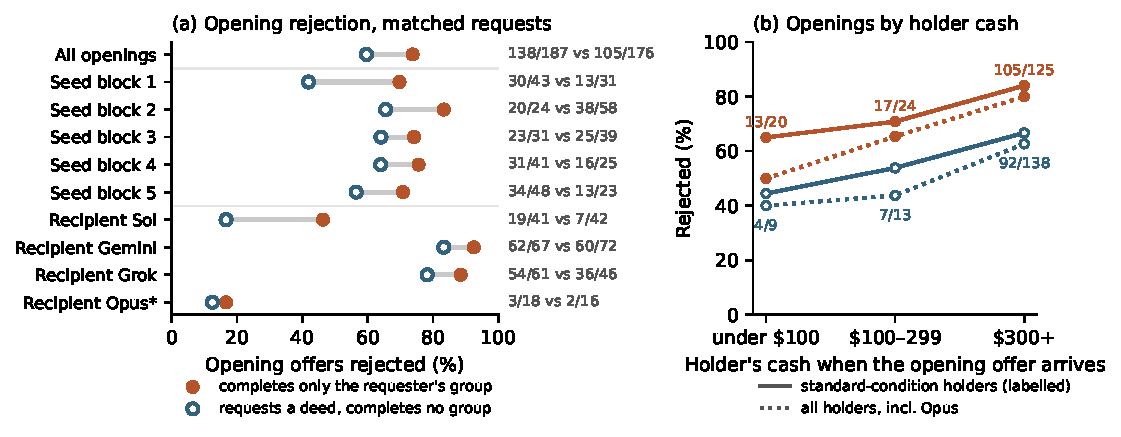
\includegraphics[width=\linewidth]{assets/fig_guard_liquidity.pdf}
\caption{The guard and its liquidity margin. (a) Share of opening offers rejected when the offer requests the deed that completes only the requester's group (filled) or requests a deed and completes no group (open), with counts, overall, by seed block and by recipient. *Opus responds under action-only recovery in 162 of its 189 trade responses. (b) The same comparison for opening offers, by the holder's cash when the offer arrives, for holders under the standard condition (solid, labelled) and for all holders (dotted).}
\label{fig:guard}
\end{figure}

The 526 threads produce 113 acceptances, 394 counters and 413 rejections. Only 32 of 524 opening offers are accepted, and 81 settlements follow at least one counter. Table~\ref{tab:matched} sorts every offer by whose group the exchange would complete and by thread position.

At the opening of a thread, recipients reject 138 of 187 completion requests (73.8\%) and 105 of 176 comparable deed requests (59.7\%). The difference of 14.1 points is positive in each seed block, at 27.9, 17.8, 10.1, 11.6 and 14.3 points, and for each recipient system (Figure~\ref{fig:guard}a). Sol shows the largest difference (19 of 41 against 7 of 42) and Gemini and Grok smaller ones from high baselines (62 of 67 against 60 of 72; 54 of 61 against 36 of 46). Opus rejects few offers of any kind but keeps the same ordering (3 of 18 against 2 of 16). An earlier comparison against all offers that complete no group gives a smaller difference, 9.9 points, because it includes 62 openings that request no deed and are rejected at 75.8\%. Being offered one's own completion barely changes the opening response: recipients reject 31 of 51 such openings, the same share as the comparator. The guard is directed at the rival's completion.

The guard operates at the threshold of a negotiation. Among later offers, completion requests and comparable deed requests are rejected at similar rates, 21 of 102 and 20 of 108. Later offers exist only where the recipient has already chosen to engage, so this is a selected population, but it shows where the difference lies. Cash concessions point the same way. Of 199 offers in which an author keeps the same non-cash terms as its previous offer and moves cash toward the recipient, recipients accept 9 of 58 that would complete only the author's group and 17 of 56 that request a deed and complete nothing. Without Opus as recipient the counts are 4 of 42 and 11 of 45. Repeated concessions in one thread are not independent observations, so we treat this as consistent with the opening pattern rather than as a separate test.

Counters themselves are generic. Of 111 counters to completion requests, 79 return the same deeds and ask for more cash, as do 81 of 110 counters to comparable deed requests. Repricing an unchanged bundle is how these agents disagree in general. What is specific to the rival's completion is the refusal to begin.

The agents' explanations name the rival. Two earlier LLM-assisted readings coded the 74 outright rejections of offers that would complete the recipient's own group. Both readers found a stated consequence for the rival in 61 of them ($\kappa=0.79$), including 27 of 38 refusals where only the recipient would complete a group. Thirty-one of the 61 agreed codes come from two games, G1 and G15, and the two readers share a model family. The codes establish what the messages and notes say, not why the agents refused. The first incident shows what such a refusal contains.

\Incident{1}{Refusing one's own monopoly (G15)}
At G15 turn 63, Sol has \$730 and Grok \$333. Sol offers its two greens for Grok's Ventnor and \$100, a swap that would complete green for Grok and yellow for Sol. Grok refuses and its note compares what each side could then build.
\Q{g15-d169-refusal-note}
Sol drops its cash request, adds Kentucky, and then adds cash of its own.
\Q{g15-d174-sweetener}
\Q{g15-d175-final-refusal}
No trade settles. Sol's note after the last refusal reads ``reassess monopoly trades when opponents need cash.'' Eighteen turns later Grok is the first player eliminated, its yellow and green blockers pass to Gemini, and Gemini wins. Grok refuses its own complete group three times because the same exchange would let Sol build first, and it keeps refusing after Sol reshapes the cash balance around that objection. Its \$600 is the price of a full first layer on green; a single legal green house costs \$200. The later elimination is one path and does not show whether refusing was the better choice.
\Source{G15 d168--176, standard first attempts. The public messages appear in each counterparty's next request.}

Prices tell a weaker version of the same story. Among offers that exchange cash for one colour-group deed and nothing else, the median ask written by the holder rises with the buyer's position in the group: 1.80 times list price when the buyer would still lack one deed (45 asks) and 2.32 when the deed completes the group (37 asks), for unmortgaged deeds. Asks to completing buyers are higher in all six seller and mortgage-status cells with at least three asks on each side. Bids move little (1.41 against 1.59 times list) and differ in sign across systems: Sol bids more for its own completion, Grok less. The closest comparison holds the seller, game and deed fixed. Seven such cases exist (Appendix~\ref{app:samedeed}). Comparing median asks, four are higher for the completing buyer, two lower and one equal; comparing first asks, five are higher, one lower and one equal. Only G4 changes direction between the two summaries, because Opus's first ask to the completing buyer exceeds its ask to the other buyer and its later asks fall as its cash falls. Both lower cases are asks made at least 19 turns apart, with the seller holding less cash at the completing asks. The asks are therefore context-sensitive, but the records identify no completion premium. The second incident shows both the pricing and its arithmetic.

\Incident{2}{One deed, two buyers, two prices (G2)}
At G2 turn 44, Sol holds Marvin Gardens and \$137, and Opus holds the other two yellows. Grok, which owns no yellow, bids \$200. Sol asks \$450, and its note prices the deed through a third party and through its own finances.
\Q{g2-d119-note}
One turn later Opus bids \$325, and Sol asks the completing buyer for more.
\Q{g2-d124-price}
Sol comes down to \$600, and Opus stops at \$450 while its own note allows about \$475. Sol keeps the deed.
\Q{g2-d128-note}
Twenty-four turns later the positions reverse. Opus, now holding \$17, gives its two yellows to Sol for two railroads and \$100. Sol completes yellow, builds two houses, sells them four turns later to pay rent, and is eliminated at turn 85; both estates pass to Gemini, which wins. Sol prices one deed at \$450 for a buyer with no yellows and \$650 for the buyer it would complete, names the resale route between them, and declines because it has mortgage reserves and no group on which to spend the proceeds. Its note at d124 says that \$520 buys ``nine yellow houses''; at \$150 each it buys three, and house costs are absent from this prompt. The concern is clear and the number is wrong.
\Source{G2 d118--128 and d196--198. d119 and d124 are standard first attempts; d118 is a Grok call whose text names a different action. Opus's d197 message is an action-only response.}

Accepting a deal is also distinct from accepting its explanation. In G19 Grok's received call offers Virginia and \$150 for States with a false claim that States is orange. Sol replies, ``States is pink, not orange---but Virginia plus \$150 works for me. Deal.'' The swap executes. The recipient corrects the premise and evaluates the terms, and the proposer's own note had said to abort the trade, so neither credulity nor successful deception is shown.

\section{Liquidity sets the terms of release}
\label{sec:liquidity}

\begin{table}[t]
\centering\small
\begin{tabular}{@{}llrrr@{}}
\toprule
& & \multicolumn{3}{c}{Holder's cash when the offer arrives}\\
\cmidrule(l){3-5}
Population & Offer & under \$100 & \$100--299 & \$300 or more\\
\midrule
Openings, standard holders & Completion request & 13/20 & 17/24 & 105/125\\
& Comparable deed request & 4/9 & 7/13 & 92/138\\
Openings, all holders & Completion request & 13/26 & 17/26 & 108/135\\
& Comparable deed request & 4/10 & 7/16 & 94/150\\
\addlinespace
Later, standard holders & Completion request & 4/28 & 5/16 & 12/24\\
& Comparable deed request & 1/7 & 4/16 & 13/52\\
Later, all holders & Completion request & 4/43 & 5/19 & 12/40\\
& Comparable deed request & 1/12 & 4/22 & 15/74\\
\bottomrule
\end{tabular}
\caption{Rejected/received offers by the holder's cash. Standard holders are recipients other than Opus, which responds under action-only recovery. The bands are descriptive strata chosen after earlier work on these records.}
\label{tab:liquidity}
\end{table}

Holders short of cash bargain differently. Pooled over both stages, holders with under \$100 reject 17 of 69 completion requests, against 120 of 175 for holders with \$300 or more. That contrast mixes three things (Table~\ref{tab:liquidity}). Forty-three of the 69 low-cash requests are later offers, which are rarely rejected at any cash level. Twenty-one go to Opus, which rejects none of them. And low cash lowers rejection of comparable deed requests as well, from 109 of 224 to 5 of 22. The cleaner view is the opening offer to a holder under the standard condition (Figure~\ref{fig:guard}b). There, rejection of completion requests falls from 84\% to 65\% as cash falls, and rejection of comparable deed requests falls from 67\% to 44\%. The difference between the two remains 17--21 points in every band. Cash need makes the holder more willing to engage with any request for a deed; it does not remove the extra refusal of a rival's completion at the opening. The systems differ. Gemini rejects all ten completion requests it receives at the opening while holding under \$100; Sol and Grok shift toward counters; Opus counters at every level. Sol's 26 low-cash completion requests come from nine threads.

Buyers act as if they know this. At the opening of a thread, 26 of 187 completion requests reach a holder with under \$100, against 10 of 176 comparable deed requests; without Opus as recipient the counts are 20 of 169 and 9 of 160. The ordering holds for every recipient system. Offers to cash-poor holders are not more generous: the median net cash offered with an opening completion request is \$165 to holders under \$100 and \$150 to holders with \$300 or more. Notes say the same. Gemini times a bid to the holder's cash in G7 (Incident~3), and Sol's G15 note plans to ``reassess monopoly trades when opponents need cash.''

Completed sales show where the guard gives way. Of 148 holder--buyer pairs, trades settle 63, and in 43 the sale completes a group for the buyer only. In 20 of those 43 the holder had under \$100 at settlement, and 12 of those 20 sellers are Opus. Swaps that complete groups for both sides look different: the median holder cash at settlement is \$594.50, and one holder of 20 had under \$100. In 14 one-sided sales the same holder had refused or countered the same buyer on an earlier turn. Its cash was lower at the sale in 13 of them, from a median of \$571.50 to \$82, and under \$100 in 8 (5 of 11 without Opus). These sequences are selected on an eventual sale, and the cash of holders in pairs that never settled also drifted down, from \$671.50 to \$516 at the median. Release followed a fall in cash more often than it followed anything else we can measure, but several holders sold with \$444 to \$774.

Short of cash is not the same as cheap. Among one-sided sales for cash alone, the six made by standard-condition holders with under \$100 settled at a median of 2.25 times list, five of them above list. The eight made by Opus with under \$100 settled at a median of 0.66, seven of them below list. The cohort cannot separate Opus's model from its response condition, but it shows that cash pressure and a low price are separable. The next incidents show the release from both sides.

\Incident{3}{A bid timed to the holder's cash, and a sale that pays for houses (G7)}
At G7 turn 25 Sol holds \$1,150 and has just bought North Carolina. It asks Grok \$650, saying it is ``already liquid.'' Grok answers with a public limit that its note does not hold.
\Q{g7-d42-final}
\Q{g7-d42-ceiling}
Sol accepts \$600. Forty-two turns later Sol has bought Park Place, built three houses on the dark blues and is left with \$84. Gemini, which needs Sol's New York Avenue to complete orange, had bid \$350 for it fifteen turns earlier and been refused. It bids \$350 again.
\Q{g7-d141-timed-bid}
\Q{g7-d142-ask-note}
Gemini pays \$700, mortgages five deeds and builds four orange houses in the same turn; Sol builds three more dark-blue houses within eight turns and wins the game. Grok's ``final'' price is an authorized bluff that settled, and nothing in the record isolates its effect. The same holder that guarded New York Avenue while liquid sells the rival's completing deed at 3.5 times list once it has houses to fund, and its note prices the sale by its own construction path and the buyer's remaining cash. The buyer, for its part, times the bid to the holder's need.
\Source{G7 d39--43 and d132--150, standard first attempts.}

\Incident{4}{A completing deed sold for a quarter of its list price (G1)}
From G1 turn 69, while holding \$453, Opus offers Boardwalk seven times in swaps that would also complete its own orange group; Grok rejects six and counters one. At turn 122, after paying a \$550 rent, Opus has \$18 and offers the mortgaged deed for cash.
\Q{g1-d306-offer}
Grok counters at \$50, Opus asks \$100, and Grok accepts.
\Q{g1-d309-accept-note}
Grok completes dark blue for a quarter of Boardwalk's list price, never redeems or builds it, and collects \$70 over the next 94 turns. Opus is eliminated four turns after the sale, owing Gemini, which wins. The holder's terms fell with its cash, from a swap for its own completion to \$100. The buyer pays above its own ceiling because the alternative is that the leader inherits the deed. Opus played under action-only recovery and left no note, so its side of the exchange shows only public messages.
\Source{G1 d305--315. Grok's responses are standard first attempts; Opus's are action-only responses.}

\Incident{5}{Distress used as a bargaining position (G13)}
At G13 turn 107 Grok has \$35, owns the three yellows and stands nine squares before Sol's Short Line, where rent is \$200. Its Ventnor is unmortgaged and would raise \$130. Grok offers Opus its mortgaged Pennsylvania Avenue.
\Q{g13-d250-insurance}
Opus counters at \$130. Grok holds at \$200; its applied note and the explanation returned with the same response differ in what they disclose.
\Q{g13-d252-floor}
\Q{g13-d252-omission}
Opus pays \$200 and \$16 of transfer interest, and completes green seven turns later at auction. Grok misses Short Line on its next roll and goes bankrupt there at turn 150; the yellows pass to Sol, and Opus wins. Grok presents its own distress as the buyer's problem and leaves out a source of cash its explanation names; under this prompt that is an authorized public bluff. Opus repeats the estate concern but does not endorse the claimed limit, and nothing shows that the omission moved the price from \$130 to \$200. The pitch's 5-in-36 is also not the single-roll 4-in-36 that Grok's own note uses.
\Source{G13 d250--253, d307 and d311. The omission appears in the returned provider explanation, a channel separate from the applied note.}

Defending against a rival's construction can also be collective. Soon after Opus sells Illinois to Grok for \$500 in G20, completing Grok's reds and leaving it \$222, Gemini addresses the table.
\Incident{6}{An appeal to withhold a rival's construction cash (G20)}
\Q{g20-d96-appeal}
Sol's note had already called Grok's reds ``cash-starved''. Grok builds one house on each red, which leaves it \$7, and then offers Vermont to Gemini for \$150.
\Q{g20-d101-refusal}
Grok mortgages Vermont for \$50 instead. Opus later bids for Grok's mortgaged deeds, telling it ``That's money you can put into more red houses right now'', and nothing settles. Grok is the first player eliminated, and Gemini wins. The appeal treats cash paid to a rival as houses on the rival's group. The record shows one public appeal, its author's follow-through and one player acting against it, not a cartel.
\Source{G20 d95--102, d129--130 and d156--160. The appeal appears in Grok's d97 request.}

\section{What the positions become}
\label{sec:positions}

\paragraph{Construction.} Trades complete 63 groups. Sol and Gemini build in their first management turn after completion on 16 of 17 and 17 of 18 groups; Opus and Grok on 7 of 15 and 3 of 13. Opponents land on these groups at similar rates in all four cases, between 3.6 and 4.8 times per 100 turns of ownership, so the difference in rent that follows reflects the rent schedule of built groups more than exposure. The construction gap has visible sources. Opus and Grok completed 7 and 5 of their groups with a mortgaged deed, against 2 and 4 for Sol and Gemini, and Opus held a median of \$268 afterwards. Of the 20 groups without first-turn construction, nine had no legal build on the group in that turn (eight held a mortgaged deed), four ended in an engine default after an invalid build request, four in a Grok call that contradicted its text, and three in a valid decision to wait, including Grok notes that defer redemption to keep cash. The gap therefore combines acquisition terms, financing choices and response conditions, and it does not rank the systems' planning.

\paragraph{Debt.}\label{sec:finance} A player whose debt exceeds its cash must raise money from a menu of mortgages and building sales or declare bankruptcy. This happens 188 times. Debtors pay in 128 episodes and are eliminated in 60. Sixty-one payments take two to ten actions, and the paying sequences contain 180 mortgages and 89 building-sale actions with no engine default. All four systems pay: Sol 30 of 31 payable debts, Gemini 37 of 38, Opus 41 of 41 under action-only recovery, Grok 20 of 21. Here payable means paid, or shown payable by an earlier engine-executed witness; 56 eliminations involve debts above a generous bound on the debtor's own sale and mortgage value, and one (G7) faced a menu that offered no building sale because the bank had no houses. The payments also preserve assets where they can. Of 68 payments that sold buildings, only two did so when the mortgages on the first menu would have covered the shortfall.

The menu lists the deeds that can be mortgaged now. A deed in a group with buildings becomes mortgageable only after those buildings are sold, and the engine presents a new menu after every action. In 19 paid episodes, spread across all four systems, the debtor sold buildings and then mortgaged a deed that had not been on the first menu. The two payable bankruptcies under the standard condition fail at exactly this step. At G12 d190 Sol owes \$500 with \$53 in cash; its note adds \$225 from house sales and \$130 from the three deeds then listed as mortgageable, concludes that \$408 is the maximum, and declares bankruptcy, omitting \$340 of red mortgages that the house sales would release. At G17 d234 Gemini owes \$550 with no cash; it adds \$500 of house salvage and \$30 for Baltic and tells the table:
\Q{g17-d234-public}
Selling the houses would have released \$375 of dark-blue mortgages. Both agents treated the first menu's list as fixed. Agents who proceeded one action at a time used the released collateral. The difference is a specific multi-step lookahead failure, not an inability to execute the step, and G17 shows that it can matter. The bankruptcy handed Park Place and Boardwalk with five houses to Sol, which held the smallest share of assets at the table and \$34 in cash, and Sol won. The third payable bankruptcy is different.

\Incident{7}{A payable debt ends in a contradictory bankruptcy (G12)}
At G12 turn 101 Grok owes Opus \$250 with \$43 in cash; its pinks carry two, two and three houses. The text of its response requests a two-house sale, and its note ends:
\Q{g12-d249-note}
The tool call the engine applied declares bankruptcy.
\Q{g12-d249-public}
Grok is eliminated and its estate passes to Opus, which wins. An earlier engine-executed check found five legal house sales that pay the debt and leave \$43; the two-house sale named in the text is legal but reaches only \$143. The note finds the route and the applied call abandons it. The record shows where the disagreement appears, in the returned response, but not which channel reflects what the system would have done.
\Source{G12 d249, standard first attempt. The public message has no later recipient exposure.}

\paragraph{Estates.} Each game's first elimination moves a whole estate, buildings intact, to one creditor, and that creditor wins 18 of the 20 games. Positions just before the transfer show that the creditor usually already led: it ranked first or tied in prior paid rent in 15 games, in a simple asset index in 15, and in buildings in 12, though in cash in only 8. In five games the creditor did not lead in assets; it won four of them, G17 among them. Inheritance in these games mostly follows an existing lead, and the five discordant games show that an estate can still change who leads. The agents bargain over that possibility directly, as the last incident shows.

\Incident{8}{A standing offer withdrawn as the seller weakens (G18)}
At G18 turn 181 Opus holds \$615 and bids \$200, then \$250, for Sol's mortgaged Pacific, which would complete its greens. Sol holds \$294 and asks \$600.
\Q{g18-d420-note}
Over the next six turns Opus says four times that its offer stands, the last time after collecting \$750 from Sol.
\Q{g18-d431-assurance}
A second \$750 rent forces Sol to sell its orange hotels and mortgage its reds, leaving \$49. Sol names Opus's price, and Opus withdraws.
\Q{g18-d442-withdrawal}
\Q{g18-d442-explanation}
Opus, holding \$2,125, redeems its two green deeds over the next four turns and bids \$150 and \$225 for Pacific; Sol asks \$450, \$350 and \$300, and nothing settles. Sol is eliminated at turn 197, its estate passes to Opus, and Opus wins. Sol states its own release rule: sell the blocker only for a large change in liquidity. Opus's returned explanation treats the seller as nearly out and its estate as likely to arrive anyway. The assurance was a public message the engine does not enforce, and nothing shows that it was insincere when made or that Sol relied on it at a cost.
\Source{G18 d419--461. Sol's responses are standard first attempts; Opus's are action-only responses, and its explanation is provider-returned text.}

\section{Discussion}
\label{sec:discussion}

\paragraph{What the agents attend to.} The completing deed is an identity-dependent externality, and the agents treat it as one. They refuse to begin negotiations over it more often than over comparable deeds, and they say why. Their attention concerns public capacity: cash, holdings, mortgages, building costs, turn order and who would inherit an estate, all facts the prompt shows or the agent can derive. The records contain many such deductions. They contain no comparable evidence about rivals' hidden beliefs, which the design does not measure. This is strategic attention in the sense of a state-linked consideration visible in choices and statements. Strategic effectiveness would require a value reference for each refusal and price, and the cohort has none~\citep{cosentino2026counterparty}.

\paragraph{Liquidity as the hinge.} The guard has a price in cash. Liquid holders refuse rivals' completions at the threshold; cash-poor holders engage, counter and sometimes sell; and buyers time their requests to the holder's need. The agents describe both sides of this exchange in their notes, from a seller declining because it has no group to build with the proceeds to a buyer bidding because the holder ``now needs cash to add houses''. Liquidity is also where execution is most visible. Paying a debt is a local task with an explicit menu and an immediate check, and the agents do it reliably. Their failures there are specific: a static sum over the first menu instead of the menu that their own first action would create. The same variable thus connects what the agents guard, when they give it up and how they meet the obligations that follow. We do not claim that cash causes release. Cash-poor holders differ in many ways, and the bands were chosen after inspection.

\paragraph{Conditions are part of the environment.} Opus counters most offers, sells most distressed completing deeds and sells them cheaply, and it played almost every decision without authored notes or a corrective retry. These records cannot separate the model from the condition. What matters for the other agents is that a ready trading partner existed: Opus opened 240 threads and sold 12 of the 20 one-sided completing deeds that changed hands from holders under \$100. Grok's conflicting calls opened another 64 threads. Each condition changed the offers the other agents received, so removing one participant's rows does not recover a clean comparison for the rest.

\paragraph{The motivating questions.} The cohort answers the example in the first motivating question directly: agents reject seemingly attractive trades because of what the trade gives an opponent, and the pattern appears in choices, not only in words. It adds evidence on opponent modelling of liquidity, contextual bargaining tactics, local financial execution and creditor succession. It does not measure calibrated beliefs about hidden information, learning caused by feedback, persuasion, the value of a price, transfer to unfamiliar opponents or the relation between general and multi-agent capability. Those remain unmeasured here, which is different from a finding that the agents lack them (Appendix~\ref{app:questions}).

\section{Related work}
\label{sec:related}

LLM bargaining has been studied in controlled two-party scenarios with explicit payoffs and tactic manipulations~\citep{bianchi2024negotiationarena}. \citet{cosentino2026counterparty} give one side ranked information about the other's preferences in a multi-issue negotiation and find that accurate counterparty modelling does not reliably improve the informed side's outcome, and that final agreements track opening anchors. Our distinction between attention and effectiveness follows theirs. Our setting has no utility reference but places bargaining inside a complete multi-player game in which a counterparty's gain affects third players and later turns.

Monopoly itself is an existing LLM testbed. AgentMonopoly compares model families, sizes and personas through trade proposals, acceptance and cash management~\citep{wu2026agentmonopoly}. FinBoardBench evaluates financial decisions across three board games including Monopoly, against fixed opponents and with models in non-thinking mode. It reports that 82 of 86 completed Monopoly deals initiated by the evaluated models finish within one round, that only a third of negotiation decisions are counters, and that the models keep buying property with little cash, which the authors read as underestimating liquidity~\citep{hu2026finboardbench}. Our cohort differs in models, harness and rules, so no comparison of model generations or interfaces follows. Descriptively, our agents counter in 394 of 920 responses, 81 of 113 settlements follow a counter, and liquidity appears as the margin on which a blocker is released rather than as a constraint ignored at purchase. The Vending-Bench Arena study joins agents' messages to simulator state and validates its communication labels with a reference set and other judge families~\citep{li2026arena}; our incidents are selected illustrations without that validation.

The economic setting is familiar. \citet{jehiel1995delay} show that identity-dependent negative externalities among potential buyers can delay a sale, and \citet{jehiel1996nuclear} study how a seller should sell when non-acquirers are harmed. In Monopoly the holder itself bears the externality of selling, which is closer to a blocker's dilemma than to a mechanism-design problem. We use these models to describe the stakes, not to claim that the agents implement an equilibrium.

\section{Limitations}
\label{sec:limits}

The cohort has five seeds, one roster, one cyclic seat order and visible model names; wins are 8, 7, 3 and 2 by system and 7, 7, 3 and 3 by seat. Every contrast here was chosen after the records were available, including the matched comparator, the cash bands and the construction window, and offers within threads and pairs are dependent. Response conditions differ by system and shape the whole table. The agents were not told the implementation's rules, and most prompts omit prices, so a wrong number in a note can be a recall error as easily as a reasoning error. The semantic codes come from two readers of one model family, one partly exposed to earlier counts, with no human check. The eight incidents were chosen after reading the records to show distinct mechanisms, and seven involve Grok, whose separate text and call channels make conflicts visible; they estimate no rate. Earlier engine-executed witnesses supply the three payable-elimination routes, the G7 menu restriction and the construction-window classification; this revision ran no game, engine, replay or model call.

\section{Conclusion}

In twenty complete games, four configured LLM systems guarded the deed that would complete a rival's colour group. They refused to begin negotiations over it more often than over comparable deeds at every level of their own cash, and they said why. Cash need made the guard negotiable: cash-poor holders countered and sold, buyers timed their requests to the holder's need, and the agents priced blockers by what the proceeds would build. The same agents paid nearly every debt they could pay, and the few payable bankruptcies share a specific lookahead error. Whether this defensive bargaining was good play is a question for a design with a value reference and varied opponents.

\begin{thebibliography}{10}\small
\bibitem[Anthropic(2026)]{anthropic2026opus55} Anthropic. What's new in Claude Opus 5.5. Documentation page, \url{https://platform.claude.com/docs/en/models/opus-5-5/whats-new-opus-5-5}, read 11 November 2026 by the drafting authors.
\bibitem[Bianchi et~al.(2024)]{bianchi2024negotiationarena} F.~Bianchi, P.~J. Chia, M.~Yuksekgonul, J.~Tagliabue, D.~Jurafsky and J.~Zou. How well can LLMs negotiate? NegotiationArena platform and analysis. In \emph{Proceedings of the 41st International Conference on Machine Learning}, PMLR 235:3935--3951, 2024.
\bibitem[Cosentino et~al.(2026)]{cosentino2026counterparty} R.~Cosentino, S.~Shekkizhar, A.~Earle and S.~Savarese. Counterparty modeling is not strategy: the limits of LLM negotiators. arXiv:2605.16575v1, 2026.
\bibitem[Hu et~al.(2026)]{hu2026finboardbench} X.~Hu, P.~Wang, J.~Miao, X.~Tao, C.~Li, Y.~Ma, J.~He, Q.~Zhang, Y.~Zou and D.~Li. FinBoardBench: benchmarking dynamic wealth management and strategic financial reasoning of LLMs via board game simulations. arXiv:2605.27896v1, 2026.
\bibitem[Jehiel and Moldovanu(1995)]{jehiel1995delay} P.~Jehiel and B.~Moldovanu. Negative externalities may cause delay in negotiation. \emph{Econometrica}, 63(6):1321--1335, 1995.
\bibitem[Jehiel et~al.(1996)]{jehiel1996nuclear} P.~Jehiel, B.~Moldovanu and E.~Stacchetti. How (not) to sell nuclear weapons. \emph{American Economic Review}, 86(4):814--829, 1996.
\bibitem[Li et~al.(2026)]{li2026arena} Z.~Li, L.~Petersson, A.~Acquisti and M.~A. Bakker. Emergent misaligned communication in long-horizon multi-agent LLM commerce. arXiv:2608.14825v3, 2026.
\bibitem[Turpin et~al.(2023)]{turpin2023unfaithful} M.~Turpin, J.~Michael, E.~Perez and S.~R. Bowman. Language models don't always say what they think: unfaithful explanations in chain-of-thought prompting. In \emph{Advances in Neural Information Processing Systems}, 2023.
\bibitem[Wu et~al.(2026)]{wu2026agentmonopoly} C.~Wu, M.~Li, M.~Marsault, X.~Huang and C.-H. Cheng. AgentMonopoly: behavioral patterns and persona control in LLM agents. arXiv:2610.29330v2, 2026.
\end{thebibliography}

\clearpage
\appendix
\section{Seven same-seller, same-game, same-deed comparisons}
\label{app:samedeed}
\begin{table}[h]
\centering\small
\begin{tabularx}{\linewidth}{@{}lXXccc@{}}
\toprule
Game, seller, deed & Asks to the completing buyer (turn: \$; seller cash) & Ask to the other buyer & Median & First ask & Gap\\
\midrule
G1 Opus, Boardwalk & t122: 100, 150; \$18 & t103: 350; \$48 & lower & lower & 19\\
G2 Sol, Marvin Gardens & t45: 600, 650; \$161 & t44: 450; \$137 & higher & higher & 1\\
G4 Opus, Boardwalk & t152: 450 (\$110); t155: 100, 175, 250 (\$60); t164: 150 (\$210) & t74: 280; \$95 & lower & higher & 78\\
G15 Opus, Baltic & t49: 120, 150, 180; t52: 100; \$8 & t49: 100; \$8 & higher & higher & 0\\
G16 Grok, Marvin Gardens & t250: 1,200; \$93 & t144: 400; \$251 & higher & higher & 106\\
G17 Grok, Mediterranean & t81: 35; \$324 & t81: 35; \$324 & equal & equal & 0\\
G20 Grok, New York & t68: 400, 400; \$16 & t65: 120; \$41 & higher & higher & 3\\
\bottomrule
\end{tabularx}
\caption{Single-deed cash asks by one seller in one game to a buyer the deed would complete and to one it would not. ``Gap'' is the number of turns between the first completing ask and the other ask. Buyers, timing and negotiation history differ within every row; no row is a controlled comparison.}
\end{table}

\section{Research-question coverage}
\label{app:questions}
\small
\begin{longtable}{@{}L{.22\linewidth}L{.42\linewidth}L{.30\linewidth}@{}}
\toprule Question & What this cohort shows & Not measured here\\\midrule\endhead
1. Strategic reasoning & Opening refusal of completion requests exceeds refusal of comparable requests in every block and for every recipient; recipients refuse their own completion with stated rival reasons & Optimality, regret, exploitability\\
2. Opponent modelling & Buyers open completion requests to cash-poor holders about twice as often; notes on rivals' building capacity, resale and estates & Calibrated beliefs about hidden information\\
3. Cooperation, negotiation and deception & Full response census; generic cash repricing; matched concessions; authorized bluff, omission, correction, withdrawal and a denial appeal in context & Persuasion effects, joint surplus, fairness, prevalence of deception\\
4. Planning and memory & Unlocked collateral used in 19 paid debts; both standard payable bankruptcies omit it; Opus's altered note condition & Benefit of memory; plan-completion rate\\
5. Adaptation and learning & Terms revised within threads; responses change with the holder's own cash & Learning caused by feedback; adaptation to unfamiliar opponents\\
6. Economic decisions and risk & Asks by buyer position; release and price by holder cash; 128 of 131 payable debts paid; building-preserving liquidation & Value of any price or reserve; risk-adjusted return\\
7. Collective dynamics & A public appeal to deny a rival construction cash with mixed follow-through; creditor succession & Coalition stability; effect of coordination\\
8. Evaluation validity & Recipient-view reconstruction; matched comparators; block and recipient replication; explicit conditions & Model ranking; performance under a repaired interface\\\midrule
A. Strategic talk versus action & Stated release rules that match population patterns; a correct concern with wrong arithmetic (G2); a found payment route abandoned by the applied call (G12) & General relation between explanation quality and play quality\\
B. General versus multi-agent capability & Nothing; the cohort has no measure of general capability & Any relationship\\
C. Skill, chance and weak opponents & Seat and seed patterns; first creditors usually already led; one payable bankruptcy handed the last-placed player a winning estate & Separate shares of skill and chance\\
\bottomrule
\end{longtable}
\end{document}
